%%% The main file. It contains definitions of basic parameters and includes all other parts.

%% Settings for single-side (simplex) printing
% Margins: left 40mm, right 25mm, top and bottom 25mm
% (but beware, LaTeX adds 1in implicitly)
\documentclass[12pt,a4paper]{report}
\setlength\textwidth{145mm}
\setlength\textheight{247mm}
\setlength\oddsidemargin{15mm}
\setlength\evensidemargin{15mm}
\setlength\topmargin{0mm}
\setlength\headsep{0mm}
\setlength\headheight{0mm}
% \openright makes the following text appear on a right-hand page
\let\openright=\clearpage

%% Settings for two-sided (duplex) printing
% \documentclass[12pt,a4paper,twoside,openright]{report}
% \setlength\textwidth{145mm}
% \setlength\textheight{247mm}
% \setlength\oddsidemargin{14.2mm}
% \setlength\evensidemargin{0mm}
% \setlength\topmargin{0mm}
% \setlength\headsep{0mm}
% \setlength\headheight{0mm}
% \let\openright=\cleardoublepage

%% Character encoding: usually latin2, cp1250 or utf8:
\usepackage[utf8]{inputenc}

%% Further useful packages (included in most LaTeX distributions)
\usepackage{amsmath}        % extensions for typesetting of math
\usepackage{amsfonts}       % math fonts
\usepackage{mathtools}		% additional math operators
\usepackage{amsthm}         % theorems, definitions, etc.
\usepackage{bbding}         % various symbols (squares, asterisks, scissors, ...)
\usepackage{bm}             % boldface symbols (\bm)
\usepackage{graphicx}       % embedding of pictures
\usepackage{fancyvrb}       % improved verbatim environment
\usepackage{natbib}         % citation style AUTHOR (YEAR), or AUTHOR [NUMBER]
\usepackage[nottoc]{tocbibind} % makes sure that bibliography and the lists
			    % of figures/tables are included in the table
			    % of contents
\usepackage{dcolumn}        % improved alignment of table columns
\usepackage{booktabs}       % improved horizontal lines in tables
\usepackage{paralist}       % improved enumerate and itemize
\usepackage[usenames]{xcolor}  % typesetting in color

\usepackage{epstopdf} %to use .eps files in the document
%%% Basic information on the thesis


\usepackage[ruled,vlined]{algorithm2e}
\usepackage{algpseudocode}
\DontPrintSemicolon

%\usepackage{algorithmic}
%%% Writing algorithms

% Thesis title in English (exactly as in the formal assignment)
\def\ThesisTitle{Key reconstruction from the inner state of RC4}

% Author of the thesis
\def\ThesisAuthor{Lukáš Sladký}

% Year when the thesis is submitted
\def\YearSubmitted{2016}

% Name of the department or institute, where the work was officially assigned
% (according to the Organizational Structure of MFF UK in English,
% or a full name of a department outside MFF)
\def\Department{Department of Algebra}

% Is it a department (katedra), or an institute (ústav)?
\def\DeptType{Department}

% Thesis supervisor: name, surname and titles
\def\Supervisor{Milan Boháček}

% Supervisor's department (again according to Organizational structure of MFF)
\def\SupervisorsDepartment{Department of Algebra}

% Study programme and specialization
\def\StudyProgramme{Mathematics}
\def\StudyBranch{Mathematical Methods of Information Security}

% An optional dedication: you can thank whomever you wish (your supervisor,
% consultant, a person who lent the software, etc.)
\def\Dedication{%
Dedication.
}

% Abstract (recommended length around 80-200 words; this is not a copy of your thesis assignment!)
\def\Abstract{%
Abstract.
}

% 3 to 5 keywords (recommended), each enclosed in curly braces
\def\Keywords{%
{RC4} {cryptoanalysis}
}

%% The hyperref package for clickable links in PDF and also for storing
%% metadata to PDF (including the table of contents).
\usepackage[pdftex,unicode]{hyperref}   % Must follow all other packages
\hypersetup{breaklinks=true}
\hypersetup{pdftitle={\ThesisTitle}}
\hypersetup{pdfauthor={\ThesisAuthor}}
\hypersetup{pdfkeywords=\Keywords}
\hypersetup{urlcolor=blue}

% Definitions of macros (see description inside)
%%% This file contains definitions of various useful macros and environments %%%
%%% Please add more macros here instead of cluttering other files with them. %%%

%%% Minor tweaks of style

% These macros employ a little dirty trick to convince LaTeX to typeset
% chapter headings sanely, without lots of empty space above them.
% Feel free to ignore.
\makeatletter
\def\@makechapterhead#1{
  {\parindent \z@ \raggedright \normalfont
   \Huge\bfseries \thechapter. #1
   \par\nobreak
   \vskip 20\p@
}}
\def\@makeschapterhead#1{
  {\parindent \z@ \raggedright \normalfont
   \Huge\bfseries #1
   \par\nobreak
   \vskip 20\p@
}}
\makeatother

% This macro defines a chapter, which is not numbered, but is included
% in the table of contents.
\def\chapwithtoc#1{
\chapter*{#1}
\addcontentsline{toc}{chapter}{#1}
}

% Draw black "slugs" whenever a line overflows, so that we can spot it easily.
\overfullrule=1mm

%%% Macros for definitions, theorems, claims, examples, ... (requires amsthm package)

\theoremstyle{plain}
\newtheorem{thm}{Theorem}
\newtheorem{lemma}[thm]{Lemma}
\newtheorem{claim}[thm]{Claim}

\theoremstyle{plain}
\newtheorem{defn}{Definition}
\newtheorem*{notation}{Notation}

\theoremstyle{remark}
\newtheorem*{cor}{Corollary}
\newtheorem*{rem}{Remark}
\newtheorem*{example}{Example}

%%% An environment for proofs

%%% FIXME %%% \newenvironment{proof}{
%%% FIXME %%%   \par\medskip\noindent
%%% FIXME %%%   \textit{Proof}.
%%% FIXME %%% }{
%%% FIXME %%% \newline
%%% FIXME %%% \rightline{$\square$}  % or \SquareCastShadowBottomRight from bbding package
%%% FIXME %%% }

%%% An environment for typesetting of program code and input/output
%%% of programs. (Requires the fancyvrb package -- fancy verbatim.)

%\DefineVerbatimEnvironment{code}{Verbatim}{fontsize=\small, frame=single}

%%% RC4 helpers
\newcommand{\K}[2]{K[{#1}...{#2}]}
\newcommand{\InvS}[1]{S^{-1}[{#1}]}


%%% The field of all real and natural numbers
\newcommand{\R}{\mathbb{R}}
\newcommand{\N}{\mathbb{N}}
\newcommand{\Z}{\mathbb{Z}}

%%% Useful operators for statistics and probability
%\DeclareMathOperator{\pr}{\textsf{P}}
%\DeclareMathOperator{\E}{\textsf{E}\,}
%\DeclareMathOperator{\var}{\textrm{var}}
%\DeclareMathOperator{\sd}{\textrm{sd}}

%%% Transposition of a vector/matrix
\newcommand{\T}[1]{#1^\top}

%%% Various math goodies
\newcommand{\goto}{\rightarrow}
\newcommand{\gotop}{\stackrel{P}{\longrightarrow}}
\newcommand{\maon}[1]{o(n^{#1})}
\newcommand{\abs}[1]{\left|{#1}\right|}
\newcommand{\dint}{\int_0^\tau\!\!\int_0^\tau}
\newcommand{\isqr}[1]{\frac{1}{\sqrt{#1}}}
\newcommand{\Mod}[1]{\ \text{mod}\ #1}
\newcommand{\FromTo}[2]{\{#1, ... , #2\} }


%%% Various table goodies
\newcommand{\pulrad}[1]{\raisebox{1.5ex}[0pt]{#1}}
\newcommand{\mc}[1]{\multicolumn{1}{c}{#1}}

\DeclarePairedDelimiter{\ceil}{\lceil}{\rceil}

%%% Rename Ensure and Require to Input and Output
\renewcommand{\algorithmicrequire}{\textbf{Input:}}
\renewcommand{\algorithmicensure}{\textbf{Output:}}

% Title page and various mandatory informational pages
\begin{document}
%%%% Title page of the thesis and other mandatory pages

%%% Title page of the thesis

\pagestyle{empty}
\hypersetup{pageanchor=false}
\begin{center}

\large

Charles University in Prague

\medskip

Faculty of Mathematics and Physics

\vfill

{\bf\Large BACHELOR THESIS}

\vfill

\centerline{\mbox{
\includegraphics[width=60mm]{../img/logo.pdf}}}

\vfill
\vspace{5mm}

{\LARGE\ThesisAuthor}

\vspace{15mm}

{\LARGE\bfseries\ThesisTitle}

\vfill

\Department

\vfill

\begin{tabular}{rl}

Supervisor of the bachelor thesis: & \Supervisor \\
\noalign{\vspace{2mm}}
Study programme: & \StudyProgramme \\
\noalign{\vspace{2mm}}
Study branch: & \StudyBranch \\
\end{tabular}

\vfill

% Zde doplňte rok
Prague \YearSubmitted

\end{center}

\newpage

%%% Here should be a bound sheet included -- a signed copy of the "bachelor
%%% thesis assignment". This assignment is NOT a part of the electronic
%%% version of the thesis. DO NOT SCAN.

%%% A page with a solemn declaration to the bachelor thesis

\openright
\hypersetup{pageanchor=true}
\pagestyle{plain}
\pagenumbering{roman}
\vglue 0pt plus 1fill

\noindent
I declare that I carried out this bachelor thesis independently, and only with the cited
sources, literature and other professional sources.

\medskip\noindent
I understand that my work relates to the rights and obligations under the Act No.~121/2000 Sb.,
the Copyright Act, as amended, in particular the fact that the Charles
University in Prague has the right to conclude a license agreement on the use of this
work as a school work pursuant to Section 60 subsection 1 of the Copyright Act.

\vspace{10mm}

\hbox{\hbox to 0.5\hsize{%
In ........ date ............	% FIXME!
\hss}\hbox to 0.5\hsize{%
signature of the author
\hss}}

\vspace{20mm}
\newpage

%%% Mandatory information page of the thesis

\openright

\vbox to 0.5\vsize{
\setlength\parindent{0mm}
\setlength\parskip{5mm}

Title:
\ThesisTitle

Author:
\ThesisAuthor

\DeptType:
\Department

Supervisor:
\Supervisor, \SupervisorsDepartment

Abstract:
\Abstract

Keywords:
\Keywords

\vss}

\newpage

%%% Dedication

\openright

\noindent
\Dedication

\newpage

\openright
\pagestyle{plain}
\pagenumbering{arabic}
\setcounter{page}{1}


%%% A page with automatically generated table of contents of the bachelor thesis

\tableofcontents

%%% Each chapter is kept in a separate file
\chapter*{Introduction}
\addcontentsline{toc}{chapter}{Introduction}

Despite its age, RC4 is still one of the most widely used stream ciphers in the world. It 




Extract the secret key from given inner state at the end of KSA. Select the best algorithm and implement it.


\TODO{co budu vyuzivat, jak se to v case vyvijelo, cemu se budu venovat, tohle resili nasledujici, ten a ten umel to a to, nasledujici clanek to vylepsil, jak, mym cilem je co( sice to udelali, ale nedodali zdrojaky, je to tam vagne popsane a tak )}
\chapter{The RC4 stream cipher}
The stream cipher RC4 was designed by Ronald L. Rivest for RSA Data Security in 1987 \cite{RS14}. It was incorporated in RSA's cryptographic library and was first commercially used in Lotus Notes. The RC4 algorithm was trade secret, but it was reverse-engineered and anonymously published in Cypherpunks mailing list  \cite{cypherpunks} in 1994. The code was accepted to be genuine as its output matched the output produced in software using licensed RC4. To avoid trademark issues, the RC4 cipher is often referred to as ARC4 or ARCFOUR, meaning Alleged RC4. 

For its simplicity and speed in software implementation it became very popular. Among implementations in products such as Skype (in modified form), Microsoft Office XP, Lotus Notes or Oracle Secure SQL, it finds application in network protocols such as WEP (Wired Equivalent Privacy), WPA (Wi-Fi Protected Access), SSL (Secure Socket Layer) and formerly in TLS (Transport Layer Security). It has been said that RC4 was the most widely used stream cipher in the world. 


TODO lepe napsat, snazili se to ohnout nejak spatne, vzali proudovou sifru a pouzili ji spatne --- wrong mode, podivat se, jak to bylo v nejakem clanku + citace \textbf{KoreK attack}
In recent years many attacks have been performed on the cipher, especially on implementations involving wrong use of the initialization vector, such as WEP. In 2015 on the basis of speculations that some state agencies have capabilities to break RC4 used in TLS has IETF published RFC 7565, which prohibited use of RC4 in TLS protocol. Similar recommendation has been issued by Microsoft and Mozilla, but RC4 is still used in many systems, mostly due to legacy reasons or ease of implementation. 

TODO citovat Milana - RC4 skro vsude u viru --- jednoducha na implementaci


\section{Description of the cipher}
RC4 is a stream cipher, encryption uses a pseudo-random stream of bits, which are combined with the plaintext using bit-wise exlusive-or (XOR), similarly to Vernam cipher. XOR is the involution, so decryption operates the same way. 
To generate the pseudo random sequence, RC4 uses secret internal state which consists of:
\begin{enumerate}
	\item a permutation of $ \Z_{N} = \FromTo{0}{N-1}$, where $ N = 2^{n} $
	\item two $n$-bit index pointers $ i,j $ used to randomize permutation table.
\end{enumerate}
The pseudo-random pointer $ j $ is secret, but $ i $ is public, its value in any stage of the stream is known. Commonly $ N = 256 $, so $ i$ and $j $ are 8-bit and the cipher is byte-oriented. Key length $ l $ is defined as the number of bytes in the key and can be in range $ 1 \leq l \leq N $.  Most applications uses the key length between 5 -- 16 bytes (corresponding to 40 -- 128 bits key).

RC4 consists of two algorithms (given bellow), Key-Scheduling Algorithm (KSA), which initializes the internal permutation involving the secret key, and Pseudo-Random Generation Algorithm (PRGA), which uses the permutation to generate pseudo-random bytes. The algorithms are described bellow. \textbf{PRGA is in fact KSA without key byte.??} Any addition related to RC4 will be addition modulo $ N $, unless specified otherwise.




\begin{algorithm}

\caption{\textbf{KSA}}
\label{ksa}
\Begin{
\textit{Initialization:} \;
$j = 0$ \;
 \textit{Scrambling:} \;
\For{$ i = 0,\cdots, N-1$}{
 $j = j + S[i] + K[i\Mod{l}]$ \\
Swap(S[i],S[j])
}
 \Return{$S$}
}
\end{algorithm}

oba vedle sebe --- neco jako minipage

\begin{algorithm}
	\Begin{
	\caption{\textbf{PRGA}}
	\label{prga}
	\textit{Initialization} \;
	$i = 0$ \;
	$j = 0$ \;
	\textit{Keystream generation loop} \;
	
	i = i + 1 \;
	j = j + S[i] \;
	Swap(S[i],S[j]) \;
	t = S[i] + S[j] \;
	\Return{$S[t]$} \;
}
\end{algorithm}



\section{RC4 sucessors/variants}


\chapter{Previous attacks}
\chapter{Theoretical analysis of the~KSA}
\TODO{je to po popisu utoku, takze to chce rict, ktery resim } 

This thesis is focused to deriving the secret key from the inner state after KSA. The permutation after the KSA algorithm is biased towards the secret key. Class of key retrieval algorithms which uses the inner state can benefit from that fact to extract complete key or information about some of its bytes. 

There are two types in biases The most likely value y-th element of permutation after complete KSA is
\TODO{In 1995 Roos observed, that 2}\\


\[ S_{N}[y] = \dfrac{y(y+1)}{2} + \K{0}{y}\]

 This equation has high probability on \TODO{formulace} first $ \sim 40 $ entries is

 It is because with hight probability happens event \TODO{event} described bellow. Similarly with last $ \sim 40 $ entries and inverse permutation. 

We can also use the fact, that with certain probability values of indices $ j_{i} $ can be found in the inner permutation or the inverse permutation and using the update rule

\[ j_{i+1} = j_{i} + S[i] + K[i\Mod{l}] \].


\TODO{Roos in 1995 } 

%[6] noticed that some of the elements of the initial permutations have a
%bias towards a linear combination of the secret key bytes. A theoretical proof of these
%biases was given by Paul and Maitra [5], later generalized by Biham and Carmeli [2].
%Thanks to our choice C[−1] = 0, these results can be given in a unified theorem as
%	follows.

Most likely value of , denoted $ S_{N}[y] $, is given by 
\[ S_{N}[y] = \dfrac{y(y+1)}{2} + \K{0}{y} \]


Hlavni myslenka, nektere klice jsou pravdepodobnejsi nez jine, z toho vnitrniho stavu!! 

We will use both facts in the key retrieval algorithm.



%%%%%%%%%%% Probability introduction %%%%%%%%%%%%
%%%%%%%%%%%%%%%%%%%%%%%%%%%%%%%%%%%%%%%%%%%%%%%%%

%%%%%%%%%%% Probability introduction %%%%%%%%%%%%
%%%%%%%%%%%%%%%%%%%%%%%%%%%%%%%%%%%%%%%%%%%%%%%%%

\chapter{Preliminaries}

\TODO{kapitolu dodelat pozdeji}
\TODO{k tomuto nejaky uvod?}
\begin{defn}
	A \defined{discrete probability space} is a pair
	$ (\Omega,\Pr) $ consisting of:
	
	\begin{enumerate}
	\item A nonempty countably infinite set $ \Omega $.
	\item A function $ \Pr: \Omega \rightarrow R $, called probability measure, 
	satisfying the following properties:
		\begin{enumerate}
			\item $  \forall \omega \in \Omega: 0 \leq Pr(\omega) \leq 1 $ %% positivity
			\item $ \sum_{\omega \in \Omega}\Pr({\omega}) = 1 $.
		\end{enumerate}
	\end{enumerate}
\end{defn}

\begin{defn}
	Let $ (\Omega,\Pr) $ be a discrete probability space. An \defined{event} $ E $ is any finite subset of $ \Omega $. The probability of $ E $ is defined as 
	$ \Pr(E) = \sum_{\omega \in E}\Pr(\omega)  $ and $ \Pr(\emptyset) = 0$.
\end{defn}

\begin{defn}
	Let $ (\Omega, \Pr) $ be a discrete probability space and $ E_{1}, E_{2} \subseteq \Omega $  where $ E_{2} \neq 0 $. Then we define \defined{conditional probability} as follows:
	
	 \[ Pr(E_{1} | E_{2}) = \dfrac{\Pr(E_{1} \cap E_{2})}{\Pr(E_{2})} \]
\end{defn}

\begin{lemma}
	\TODO{zakladni vztahy}
	\[ \Pr(A \cup B) = \Pr(A) + \Pr(B) - \Pr(A \cap B) \]
	\[\Pr(\complem{A}) = 1-\Pr(A)\]
\end{lemma}


\begin{thm}
	(The law of total probability)
	
	\begin{equation}\label{totalProb}
	\Pr(E) = \sum_{n}\Pr(A \cap B_{n}) = \sum_{n}\Pr(A \, | \, B_{n})\Pr(B_{n})
	\end{equation}
	
	
	
	\TODO{veta o uplne pravdepodobnosti}
\end{thm}

\begin{defn}
	\TODO{\textbf{Uniform distributio}n takto nebo musim zavadet jevy jako zobrazeni?}
	$ \forall \omega \in \Omega : \Pr(\omega) = \dfrac{1}{|\Omega|} $
\end{defn}

\begin{defn}
Two events $ A $ and $ B $ are independent (often written as $ A \perp B  $) if and only if their joint probability equals the product of their probabilities:

\[ \Pr{(A \cap B)} = \Pr{(A)}\Pr{(B)}. \]
\end{defn} 

\begin{notation}
		\red{$ \complem{A} $ is complementary event to $ A $}
\end{notation}
	



%%%%%%%%%%% Notations                %%%%%%%%%%%%
%%%%%%%%%%%%%%%%%%%%%%%%%%%%%%%%%%%%%%%%%%%%%%%%%
\section{Notations and basic assumptions}

\begin{notation}
	Let $ K $ be the array of key bytes \red{with} length $ l $. We will \red{denote} 
	
	\[\K{a}{b} \coloneqq \sum\limits_{i=a}^{b}K[i \Mod{l}] 	\]
	
	The indice $ j $ in $ r $-th round of the KSA will be noted $ j_{r} $, the permutation after $ r $ rounds will be $ S_{r} $. Therefore $ S_{N} $ is the permutation after complete KSA.
	
	$ 	\InvS $ will stand for the inverse of the permutation $ S $, i.e. $ \forall y \in \FromTo{0}{N-1}: S[y] = v \Rightarrow \InvS[v] = y$.
	

	\red{Mozna jeste $ K[a] = K[a \Mod{l}] $}
\end{notation}


%%%%%%%%%%% Prvni bias %%%%%%%%%%%%%%%%%%%%%%%%%%
%%%%%%%%%%%%%%%%%%%%%%%%%%%%%%%%%%%%%%%%%%%%%%%%%

\section{Roos bias}


	%%% Prerekvizita vety 
	\begin{lemma}
		\red{prerekvizita vety 1}
		Assume that the index $ j $ takes its value from $ \Z_{N}  $ uniformly at random at each round of the KSA. Then $ \forall y \in \Z_{N} $:
		
		\[ \Pr\Big(j_{y+1} = \dfrac{y(y+1)}{2} + \K{0}{y} \Big) 
		\approx 
		\Big(\dfrac{N-1}{N}\Big)^{1+\frac{y(y+1)}{2}} + \dfrac{1}{N}
		\]
		
	\end{lemma}		
	\begin{proof}
		Let $ E_{y} $ denote the event that $ j_{y+1} = \sum_{x=0}^{y}(y + K[x mod l])$
	\end{proof}	
	
	%%% Prerekvizita vety 	
	\begin{lemma}
		\TODO{prerekvizita vety 1}
	\end{lemma}



	
	\begin{thm}{\cite{GoMa}}
		Assume that during the KSA the index j takes its values uniformly at random from $ \Z_{N} $. Then $ \forall 0 \leq i \leq r-1, 1 \leq r \leq N $
		
		\[ \Pr(S_{r}[i] = \K{0}{i} + \dfrac{i(i+1)}{2})   \geq (\dfrac{N - i}{N})(\dfrac{N-1}{1})^{\frac{i(i+1)}{2}+r}+\dfrac{1}{N} \]
	\end{thm}
	
	\begin{proof}
		\TODO{dukaz}
	\end{proof}
	
	\begin{cor}
	\TODO{zobecneni na posledni kolo nebo predchozi vetu rovnou smerovat tam?}
\end{cor}
	
\TODO{tabulka s aktualnimi hodnotami } 

\TODO{to same pro InvS} 


\begin{thm}
	After the complete KSA, 
	\[  \Pr(S_{N}[S_{N}[y]] = \K{0}{i} + \dfrac{i(i+1)}{2}) \approx  \]
	
	clanek 4, appendix, na zacatku graf
\end{thm}

\TODO{tabulka s aktualnimi hodnotami, dukaz}


\begin{notation}
		\[  C_{y} = S_{N}[y] - \dfrac{y(y+1)}{2} \]
\end{notation}

\TODO{zobecneni na sekvence}


\TODO{inverzni sekvence}

\TODO{vyyiti tohoto na ziskani klice - rovnice} 


\section{Substracting equations}

Let $i_{1} < i_{2} $. If $ C_{i_{1}} = \K{0}{i_{1}} $ and $ C_{i_{2}} = \K{0}{i_{2}} $, then we can substract the values and get
\[ C_{i_{2}} - C_{i_{1}} = \K{0}{i_{2}} - \K{0}{i_{1}} = \K{i_{1} + 1}{i_{2}}	\].

This holds with the product of the individual probabilities of $ C_{i} $



%%%%%%%%%%% Druhy bias               %%%%%%%%%%%%
%%%%%%%%%%%%%%%%%%%%%%%%%%%%%%%%%%%%%%%%%%%%%%%%%
\section{Useful distributions for The Key Recovering Algorithm}

\begin{defn}
If $ j_{i} = S[i] $, we call this as event 1 has occured for index $ i $, and denote as $ E_{1} $.
\end{defn}

\begin{thm}
\[	P(S[i] = j_{i}) \geq (1-\dfrac{1}{N})^{i}(1-\dfrac{i-1}{N})(1-\dfrac{1}{N})^{N-i-1}+ \dfrac{1}{N} \]
\end{thm}

\begin{defn}
	If $ j_{i} = S[i] $, we call this as event 1' has occured for index $ i $, and denote as $ E'_{1} $.
\end{defn}

\begin{thm}
	\[	P(S^{-1}[i] = j_{i}) \geq (\dfrac{i}{N})(1-\dfrac{1}{N})^{N-1}+ \dfrac{1}{N}\]
\end{thm}


\begin{proof}
		$ (1-\dfrac{1}{N})^{i}(\dfrac{i}{N})(1-\dfrac{1}{N})^{N-i-1}+ \dfrac{1}{N} $
\end{proof}

\begin{thm}
	$ P(S[i] = j_{i} \vee S^{-1}[i] = j_{i}) $ used for BuildKeyTable algorithm in paper 1
\end{thm}


\TODO{ $ P(S[S[i]] = j_{i}) $ - dukazy nikde nejsou...}

\TODO{ $ P(S^{-1}[S^{-1}[i]] = j_{i}) $}

\TODO{ $ P(S[S[S[i]] = j_{i}) $}

\begin{figure}
\centering
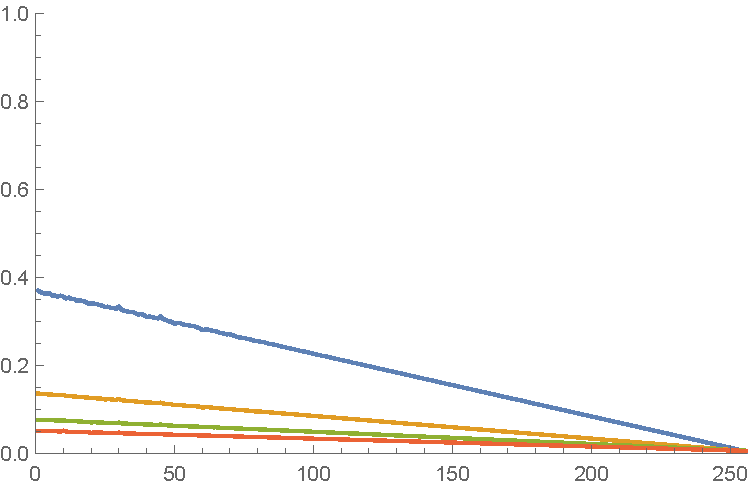
\includegraphics[width=0.7\linewidth]{img/all}
\caption[All]{hallo}
\label{fig:all}
\end{figure}


\TODO{experimentalne... rychle to konverguje}




\chapter{Going back to permutation after KSA}
Nekam napsat, ze to jde snadno ukrást v paměti, když vím detaily implementace (hledam 256 prvků, co jsou permutace). - kdyztak napsat milanovi


The internal permutation of RC4 is easy to obtain from the memory. 

Útoky state recovery attacks kombinované s tímto


\begin{itemize}
	\item I have state, $ i,j $, number of rounds. 
	\item I have state, $ i,j $, not number of rounds. 
	\item I have state, number of rounds. 
\end{itemize}



\begin{algorithm}[]
	\SetKwInOut{Input}{input}
	\SetKwInOut{Output}{output}
	
	\Input{ Number of rounds $ R $ \newline 
		    Internal state $ S_{R} $ 
		  }
	\Output{Candidates for $ S_{N} $}
	
	\Begin{
		\caption{\textbf{PRGAreverse}}
		\label{prgareverse}

		\For{$ j_{R} \in \FromTo{0}{N-1} $}{
			$ i = i_{C} $ \;
			$ j = R \Mod{N}$ \;
			$ S = S_{R} $ \;
 			$ r = R $ \;
			\While{$ r > 0 $}{
				Swap($ S[i] $,$ S[j] $)	\;
				$ j=j-S[i] $ \;
				$ i = i - 1 $ \;
				$ r = r-1 $ \;
			}
			\If{j = 0}{try $ S $ as a candidate to $ S_{N} $} \;
			\textbf{TODO Jak formulovat output?}
		}
	
	}
\end{algorithm}

If $ i,j $ are known, the algorithm will be similar, only the for loop will disappear and the condition for while loop will be $ i = j = 0 $. On the other side if neither $ j $ nor $ R $ values are known, we need to test all values of $ i,j $ pointers. If the condition $ i = j = 0 $ is fulfilled, it doesn't necessarily mean, that it is the only permutation candidate for chosen $ i,j $. The pointers could be equeal zero also during the PRGA. 
\chapter{The Key Recovering Algorithm}

Tady bych chtel popsat ten, ktery ve finale pouziju. Nebo vsechny?


\TODO{Some keys are more probable than others, we will sort them according to weight and try first $ nc $ number of candidates? Dat to tam?}\label{key}

\chapter*{Conclusion}
\addcontentsline{toc}{chapter}{Conclusion}


%%% Bibliography
%%% Bibliography (literature used as a source)
%%%
%%% We employ bibTeX to construct the bibliography. It processes
%%% citations in the text (e.g., the \cite{...} macro) and looks up
%%% relevant entries in the bibliography.bib file.
%%%
%%% The \bibliographystyle command selects, which style will be used
%%% for references from the text. The argument in curly brackets is
%%% the name of the corresponding style file (*.bst). Both styles
%%% mentioned in this template are included in LaTeX distributions.

\bibliographystyle{plainnat}    %% Author (year)
%\bibliographystyle{unsrt}     %% [number]
	


\renewcommand{\bibname}{Bibliography}

%%% Generate the bibliography. Beware that if you cited no works,
%%% the empty list will be omitted completely.

\bibliography{bibliography}

%%% If case you prefer to write the bibliography manually (without bibTeX),
%%% you can use the following. Please follow the ISO 690 standard and
%%% citation conventions of your field of research.

% \begin{thebibliography}{99}
%
% \bibitem{lamport94}
%   {\sc Lamport,} Leslie.
%   \emph{\LaTeX: A Document Preparation System}.
%   2nd edition.
%   Massachusetts: Addison Wesley, 1994.
%   ISBN 0-201-52983-1.
%
% \end{thebibliography}



%%% Figures used in the thesis (consider if this is needed)
%\listoffigures

%%% Tables used in the thesis (consider if this is needed)
%%% In mathematical theses, it could be better to move the list of tables to the beginning of the thesis.
%\listoftables

%%% Abbreviations used in the thesis, if any, including their explanation
%%% In mathematical theses, it could be better to move the list of abbreviations to the beginning of the thesis.
%\chapwithtoc{List of Abbreviations}

%%% Attachments to the bachelor thesis, if any. Each attachment must be
%%% referred to at least once from the text of the thesis. Attachments
%%% are numbered.
%%%
%%% The printed version should preferably contain attachments, which can be
%%% read (additional tables and charts, supplementary text, examples of
%%% program output, etc.). The electronic version is more suited for attachments
%%% which will likely be used in an electronic form rather than read (program
%%% source code, data files, interactive charts, etc.). Electronic attachments
%%% should be uploaded to SIS and optionally also included in the thesis on a~CD/DVD.
%\chapwithtoc{Attachments}

\openright
\end{document}
